\documentclass{article}
\usepackage{tkz-graph}
\usepackage{paralist}
\pagestyle{empty}
\usetikzlibrary{patterns}

\begin{document}

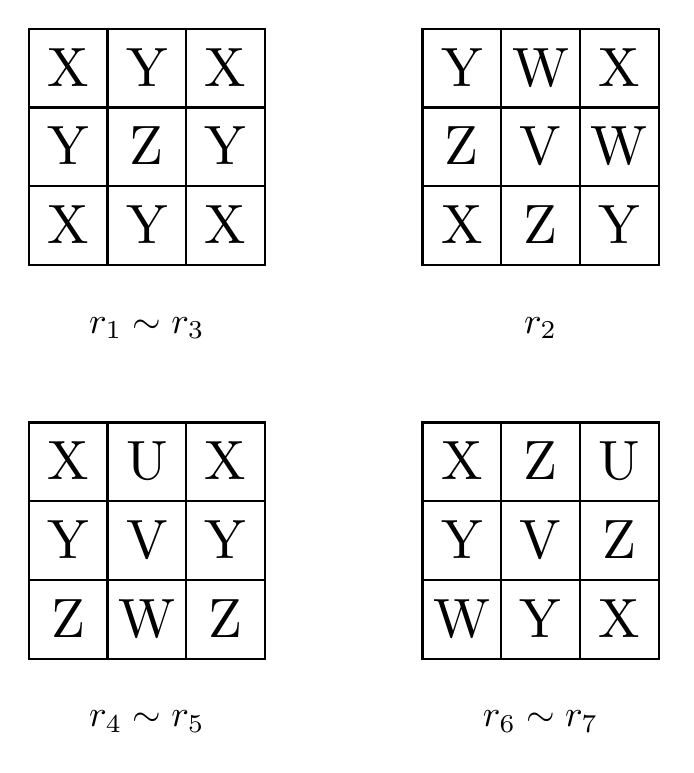
\begin{tikzpicture}

\draw[thick] (-2,4) rectangle (-1,5);
\draw[thick] (-2,5) rectangle (-1,6);
\draw[thick] (-2,6) rectangle (-1,7);
\draw[thick] (-1,4) rectangle (0,5);
\draw[thick] (-1,5) rectangle (0,6);
\draw[thick] (-1,6) rectangle (0,7);
\draw[thick] (0,4) rectangle (1,5);
\draw[thick] (0,5) rectangle (1,6);
\draw[thick] (0,6) rectangle (1,7);

\draw (-1.5,6) node[anchor=north, scale=2] {Y};
\draw (-1.5,5) node[anchor=north, scale=2] {X};
\draw (-0.5,6) node[anchor=north, scale=2] {Z};
\draw (-0.5,5) node[anchor=north, scale=2] {Y};
\draw (0.5,5) node[anchor=north, scale=2] {X};
\draw (0.5,6) node[anchor=north, scale=2] {Y};
\draw (-0.5,7) node[anchor=north, scale=2] {Y};
\draw (0.5,7) node[anchor=north, scale=2] {X};
\draw (-1.5,7) node[anchor=north, scale=2] {X};

\draw (-0.5,3.5) node[anchor=north, scale=1.33] {$r_1 \sim r_3$};

\draw[thick] (3,4) rectangle (4,5);
\draw[thick] (3,5) rectangle (4,6);
\draw[thick] (3,6) rectangle (4,7);
\draw[thick] (4,4) rectangle (5,5);
\draw[thick] (4,5) rectangle (5,6);
\draw[thick] (4,6) rectangle (5,7);
\draw[thick] (5,4) rectangle (6,5);
\draw[thick] (5,5) rectangle (6,6);
\draw[thick] (5,6) rectangle (6,7);

\draw (3.5,6) node[anchor=north, scale=2] {Z};
\draw (3.5,5) node[anchor=north, scale=2] {X};
\draw (4.5,6) node[anchor=north, scale=2] {V};
\draw (4.5,5) node[anchor=north, scale=2] {Z};
\draw (5.5,5) node[anchor=north, scale=2] {Y};
\draw (5.5,6) node[anchor=north, scale=2] {W};
\draw (4.5,7) node[anchor=north, scale=2] {W};
\draw (5.5,7) node[anchor=north, scale=2] {X};
\draw (3.5,7) node[anchor=north, scale=2] {Y};

\draw (4.5,3.5) node[anchor=north, scale=1.33] {$r_2$};

\draw[thick] (-2,-1) rectangle (-1,0);
\draw[thick] (-2,0) rectangle (-1,1);
\draw[thick] (-2,1) rectangle (-1,2);
\draw[thick] (-1,-1) rectangle (0,0);
\draw[thick] (-1,0) rectangle (0,1);
\draw[thick] (-1,1) rectangle (0,2);
\draw[thick] (0,-1) rectangle (1,0);
\draw[thick] (0,0) rectangle (1,1);
\draw[thick] (0,1) rectangle (1,2);

\draw (-1.5,1) node[anchor=north, scale=2] {Y};
\draw (-1.5,0) node[anchor=north, scale=2] {Z};
\draw (-0.5,1) node[anchor=north, scale=2] {V};
\draw (-0.5,0) node[anchor=north, scale=2] {W};
\draw (0.5,0) node[anchor=north, scale=2] {Z};
\draw (0.5,1) node[anchor=north, scale=2] {Y};
\draw (-0.5,2) node[anchor=north, scale=2] {U};
\draw (0.5,2) node[anchor=north, scale=2] {X};
\draw (-1.5,2) node[anchor=north, scale=2] {X};

\draw (-0.5,-1.5) node[anchor=north, scale=1.33] {$r_4 \sim r_5$};

\draw[thick] (3,-1) rectangle (4,0);
\draw[thick] (3,0) rectangle (4,1);
\draw[thick] (3,1) rectangle (4,2);
\draw[thick] (4,-1) rectangle (5,0);
\draw[thick] (4,0) rectangle (5,1);
\draw[thick] (4,1) rectangle (5,2);
\draw[thick] (5,-1) rectangle (6,0);
\draw[thick] (5,0) rectangle (6,1);
\draw[thick] (5,1) rectangle (6,2);

\draw (3.5,1) node[anchor=north, scale=2] {Y};
\draw (3.5,0) node[anchor=north, scale=2] {W};
\draw (4.5,1) node[anchor=north, scale=2] {V};
\draw (4.5,0) node[anchor=north, scale=2] {Y};
\draw (5.5,0) node[anchor=north, scale=2] {X};
\draw (5.5,1) node[anchor=north, scale=2] {Z};
\draw (4.5,2) node[anchor=north, scale=2] {Z};
\draw (5.5,2) node[anchor=north, scale=2] {U};
\draw (3.5,2) node[anchor=north, scale=2] {X};

\draw (4.5,-1.5) node[anchor=north, scale=1.33] {$r_6 \sim r_7$};


\end{tikzpicture}

\end{document}